\subsection[Alberi decisionali]{Alberi decisionali}


\begin{frame}
	
	\frametitle{Gli alberi decisionali}
	
	\begin{figure}[!htbp]
		\centering
		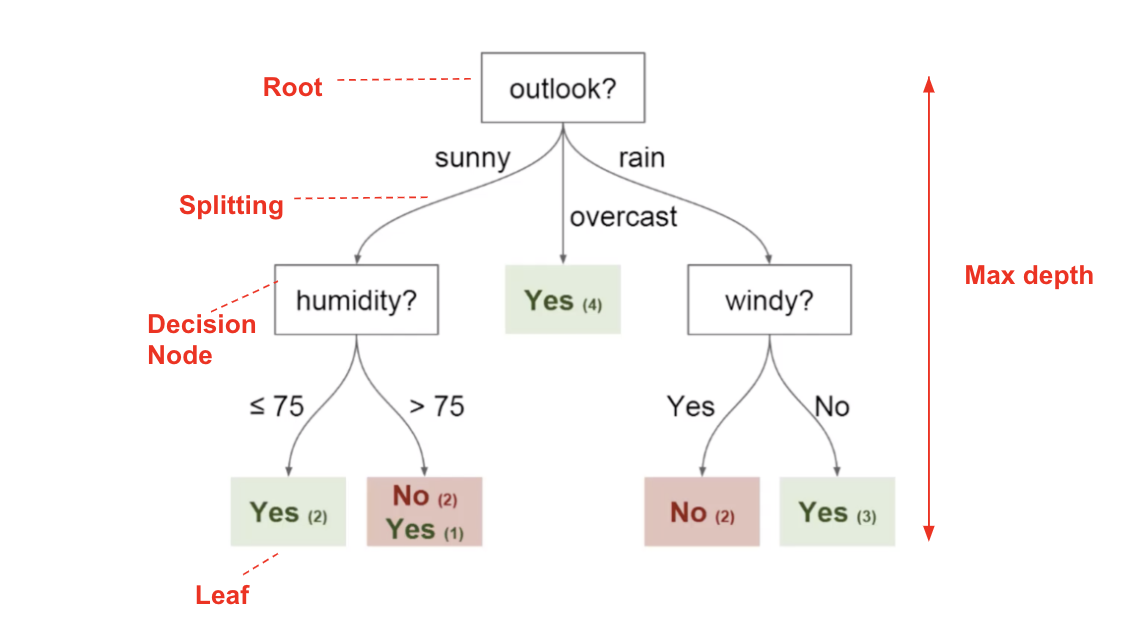
\includegraphics[width=0.95\linewidth]{images/supervised/decision_trees/decision_trees.png}
		\caption{To Play or Not To Play?}
	\end{figure}
	
\end{frame}


\begin{frame}
	
	\frametitle{Le ragioni che hanno portato agli alberi decisionali}
		
		Ricapitoliamo alcuni pro e contro del classificatore k-NN:
		\pause
		\begin{itemize}
			\item in dimensioni ridotte è in realtà abbastanza potente (gestisce confini decisionali non lineari e gestire problemi multi-classe)
			\pause
			\item utilizza molto spazio di archiviazione (training-set in memoria)
			\pause
			\item è necessaria una buona metrica della distanza
			\pause
			\item assume che input simili abbiano vicini simili%. Ciò implicherebbe che i punti dati di varie classi non siano distribuiti in modo casuale nello spazio, ma compaiano invece in gruppi di compiti di classe più o meno omogenei
			%\item sebbene esistano strutture dati efficienti che consentono una ricerca più rapida del vicino più vicino, è importante ricordare che l'obiettivo finale del classificatore è semplicemente quello di fornire una previsione accurata
			\pause
			\item immagina un problema di classificazione binaria con etichette di classe positive e negative. Se sapessi che un punto di prova si trova in un cluster di 1 milione di punti con tutte le etichette positive, sapresti che i suoi vicini saranno positivi anche prima di calcolare le distanze per ciascuno di questi milioni di distanze. È quindi sufficiente sapere semplicemente che il test point è un'area in cui tutti i vicini sono positivi, la sua esatta identità è irrilevante.
		\end{itemize}
		\pause
		\textit{Gli \textbf{alberi decisionali} cercano di sfruttare soprattutto quest'ultimo aspetto.}

\end{frame}


\begin{frame}
	
	\frametitle{Gli alberi decisionali}
	
	Innanzitutto distinguiamo due diverse tipologie di alberi decisionali, a seconda del tipo di predizione per il quale sono costruiti:
	\begin{itemize}
		\item \textbf{alberi di classificazione}: per predire variabili di tipo categorico
		\item \textbf{alberi di regressione}: per predire variabili di tipo quantitativo
	\end{itemize}
	\  \\
	Gli \textbf{alberi decisionali} risolvono alcuni problemi del k-NN: non memorizzano il training set, invece lo utilizzano per costruire una struttura ad albero che divide ricorsivamente lo spazio in regioni con etichette simili:
	\begin{itemize}
		\item[--] il nodo radice dell'albero rappresenta l'intero set di dati
		\item[--] questo insieme viene quindi diviso all'incirca a metà lungo una dimensione da una semplice soglia $t$
		\item[--] tutti i punti che hanno un valore della feature $\geq t$ finiscono nel nodo figlio destro, tutti gli altri nel nodo figlio sinistro
	\end{itemize}

\end{frame}


\begin{frame}
	
	\frametitle{Gli alberi decisionali: la soglia di split}

	\begin{itemize}
		\item[--] la soglia $t$ e la dimensione vengono scelte in modo che i nodi figlio risultanti siano \textbf{più puri} in termini di appartenenza alla classe
		\item[--] idealmente tutti i punti positivi cadono in un nodo figlio e tutti i punti negativi nell'altro
			\begin{itemize}
				\item[--] se questo è il caso, l'albero è definitivo
				\item[--] in caso contrario, i nodi foglia vengono nuovamente divisi fino a quando alla fine tutte le foglie sono pure (cioè tutti i suoi punti dati contengono la stessa etichetta) o non possono essere ulteriormente suddivisi (nel raro caso con due punti identici di etichette diverse)
			\end{itemize}
	\end{itemize}
	
	\begin{figure}[!htbp]
		\centering
		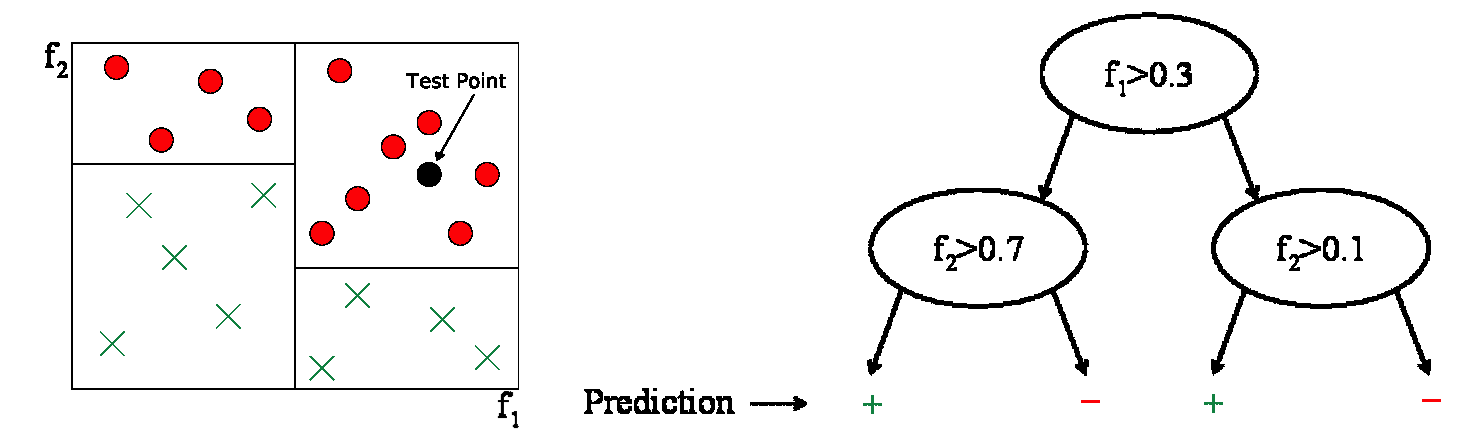
\includegraphics[width=0.8\linewidth]{images/supervised/decision_trees/binary_decision_tree.png}
		%\caption{Stripe Radar for Fraud Detection}
	\end{figure}

\end{frame}


\begin{frame}
	
	\frametitle{Gli alberi decisionali: decision boundaries}
	
	Le istanze sono di solito rappresentate utilizzando attributi discreti
	\begin{itemize}
		\item valori tipici: nominale/categorico (\{red, yellow, green\})
		\item valori numerici
			\begin{itemize}
				\item[--] discretizzazione
				\item[--] utilizzo di thresholds per i nodi di split
			\end{itemize}
	\end{itemize}
	In pratica, lo spazio delle istanze si divide in rettangoli paralleli agli assi
	\begin{figure}[!htbp]
		\centering
		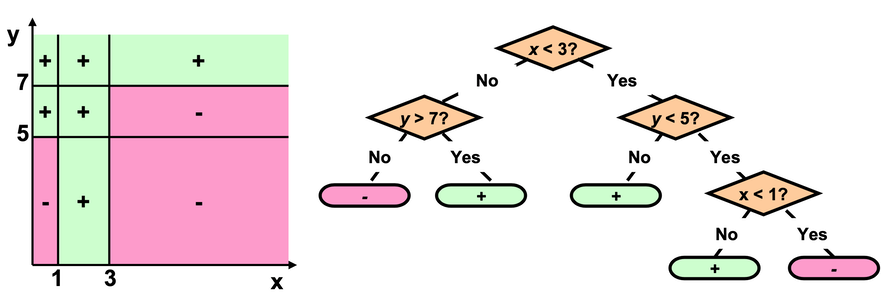
\includegraphics[width=1.00\linewidth]{images/supervised/decision_trees/example_decision_boundaries.png}
%		\caption{To Play or Not To Play?}
	\end{figure}
\end{frame}


\begin{frame}
	
	\frametitle{Gli alberi decisionali: vantaggi rispetto a k-NN}
	
	Gli \textbf{alberi decisionali} hanno \textbf{diversi vantaggi} rispetto al k-NN:
	\pause	
	\begin{enumerate}
		\item una volta costruito l'albero, il training set non deve essere mantenuto in memoria%.\\
			%Infatti possiamo semplicemente memorizzare quanti punti di ciascuna label sono finiti in ogni foglia - in genere questi sono puri, quindi dobbiamo solo memorizzare la label di tutti i punti
		\pause
		\item gli alberi decisionali sono molto veloci nell'esecuzione del test.\\
			Questo poiché gli input del test devono semplicemente attraversare l'albero fino ad arrivare ad una foglia - la previsione è la label principale della foglia
		\pause
		\item gli alberi decisionali non richiedono metriche perché le suddivisioni si basano su soglie sulle features e non su distanze
	\end{enumerate}
	
\end{frame}


\begin{frame}
	
	\frametitle{Gli alberi decisionali: osservazioni}
	
	\begin{itemize}
		\item \textbf{Nuovo obiettivo}, costruire un albero che sia:
			\begin{itemize}
				\item[--] il più possibile compatto (\href{https://it.wikipedia.org/wiki/Rasoio\_di\_Occam}{\textit{Occam's Razor}})
				\item[--] ha solo foglie pure
			\end{itemize}
		\pause
		\item \textbf{Domanda}: è sempre possibile trovare un albero coerente?\\
			Sì, se e solo se due vettori di input non hanno caratteristiche identiche con etichette diverse
		\pause
		\item \textbf{Notizia cattiva}: trovare un albero di dimensioni minime è un problema \href{https://it.wikipedia.org/wiki/NP-difficile}{\textit{NP-Hard}}!
		\pause
		\item \textbf{Notizia buona}: possiamo approssimarlo in modo molto efficace con una strategia golosa (greedy), che applica il divide-et-impera.\\
			Basta continuare a splittare i dati percorrendo gli split che minimizzano il valore di una \textbf{misura di impurità} che misura la purezza delle labels tra i nodi figli
				\begin{itemize}
					\item[--] decisione principale: l'attributo da scegliere
					\item[--] decisione desiderata: attributi che splittano gli esempi in insiemi che sono relativamente ``puri'' (portare più rapidamente possibile ad un nodo foglia)
				\end{itemize}
	\end{itemize}
	
\end{frame}


\subsubsection[Build-DT]{\textit{Build-DT}}
\begin{frame}
	
	\frametitle{Gli alberi decisionali: algoritmo}

	\begin{block}{function Build-DT(D, Features):}
		\begin{scriptsize}
		\begin{algorithm}[H]
%			\KwData{All examples}
%			\KwResult{A decision tree}
			\eIf{all examples have the same label}{
				return (leaf node with label)\;
				}{
				\uIf{Features = $\varnothing$}{
					return (leaf node with majority label)\;
				}
				\Else{
					choose the \underline{best feature $A$} as root (see impurity functions)\\
					\ForEach{value $v$ of $A$}{
						create a fork from root node with condition $A=v$\\
						
						
						\uIf{$\{x \in D: x.A=v\} = \varnothing$}{
							return (leaf node with majority label)\;
						}
						\Else{
							Build-DT($\{x \in D: x.A=v\}$, Features$\sim\{A\}$)
						}
					}
				}
			}
	%	 \caption{How to write algorithms}
		\end{algorithm}	
		\end{scriptsize}

	\end{block}


\end{frame}


\subsubsection[ID3]{\textit{ID3}}
\begin{frame}
	
	\frametitle{Gli alberi decisionali: misure di impurità}
	
	Esistono diverse \textbf{misure di impurità} con il quale possiamo decidere di selezionare la migliore feature all'interno del \textit{Build-DT}:
	\begin{itemize}
		\item Gini Impurity -- Indice di eterogeneità di Gini \textit{(CART)}
		\item Information Gain -- Guadagno di informazione \textit{(ID3, C4.5)}
		\item Variance Reduction -- Riduzione della varianza \textit{(CHAID)}
	\end{itemize}
	
	\pause
	Ci focalizzeremo sull'\textbf{Information Gain}, perché è la più intuitiva e riesce a render conto del come un albero di decisione sia in grado di rilevare una \textit{capacità predittiva migliore} per un determinato split.
	\pause
	\newlinedouble
	Negli anni Settanta, Ross Quinlan aveva creato un algoritmo per gli alberi di decisione basato sull'information gain, \textbf{ID3}, che è ancora molto diffuso grazie alla versione \textbf{C4.5} (è un aggiornamento più recente dell'algoritmo).
	Un'implementazione Java open source dell'algoritmo C4.5 è stata sviluppata per \href{https://www.cs.waikato.ac.nz/ml/weka/index.html}{Weka}. È disponibile su github al seguente \href{https://github.com/Waikato/weka-3.8/blob/master/weka/src/main/java/weka/classifiers/trees/J48.java}{link}.

\end{frame}


\begin{frame}
	
	\frametitle{Information gain}
	
	L'\textbf{information gain} si basa sulla formula della entropia informativa, una formula generale che descrive il valore atteso dalle informazioni contenute in un messaggio.
	
	Entropia, un concetto basato sulla teoria dell’informazione
	\begin{itemize}
		\item misura l’impurità di uno split
		\item seleziona l’attributo che massimizza la riduzione di entropia
	\end{itemize}
	
	\begin{figure}[!htbp]
		\centering
		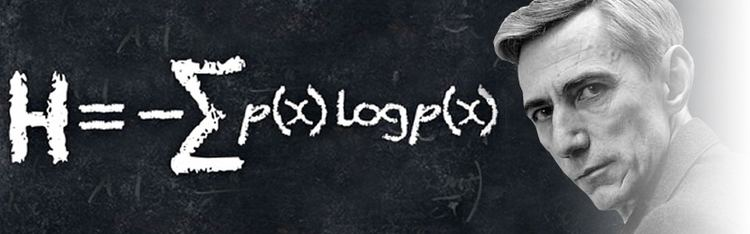
\includegraphics[width=0.9\linewidth]{images/supervised/decision_trees/claude-shannon.jpg}
		\caption{Claude Shannon, il padre della teoria dell'informazione}
	\end{figure}
	
\end{frame}


\begin{frame}
	
	\frametitle{Information Gain}
	
	%\begin{scriptsize}	
	
	\textbf{Dati}:
	\begin{itemize}
		\item $D$: l'insieme dei dati di inputs con $c$ possibili classi
		
		\begin{itemize}
			\item[--] $D=\left \{ \left ( \mathbf{x}_1,y_1 \right ),\dots,\left ( \mathbf{x}_n,y_n \right ) \right \}, y_i\in\left \{ 1,\dots,c \right \}$
			\item[--] Sia $D_k\subseteq D$ dove $D_k=\left \{ \left ( \mathbf{x},y \right )\in D:y=k \right \}$ (gli input con label $k$)
			\item[--] $D=D_1\cup \dots \cup D_c$
			\item[--] $D_i\cap D_j=\varnothing \quad \forall i \neq j \text{ con }i, j \in\left \{ 1,\dots,c \right \}$
		\end{itemize}
		\item $p_\ell=\frac{\left | D_\ell \right |}{\left | D \right |}\leftarrow \textrm{frazione degli inputs in } D \textrm{ con label } \ell$
	\end{itemize}
	
	L'\textbf{entropia} è data da:
	
	\begin{itemize}
		\item $H(D)=-\sum_{i=1}^c p_i log_2 p_i$
		\item $H(D, F = k)= -\sum_{\ell=1}^c p_{F=k, \ell} \text{ } log_2 p_{F=k, \ell} \text{ }$ dove:
		\begin{itemize}
			\item[--] la feature $F$ può assumere valori $\in \{ 1,\dots,K \}$
			\item[--] $p_{F=k, \ell}=\frac{\left | D_{F = k \text{ di classe } \ell} \right |}{\left | D_{F = k} \right |}\leftarrow \textrm{frazione degli inputs in } D_{F = k} \textrm{ con label } \ell$
		\end{itemize}
	\end{itemize}
	
	L'\textbf{information gain} della feature $F$ è pari a:
	\begin{itemize}
		\item $Gain(D, F)= -H(D) -\sum_{k=1}^K \frac{|D_{F=k}|}{|D|} \dot H(D, F = k)$
	\end{itemize}	
	
	%\end{scriptsize}
\end{frame}


\begin{frame}
	\frametitle{Entropia}
	
	\begin{columns}
	
			\column{0.4\linewidth}
			\begin{figure}[!htbp]
				\centering
				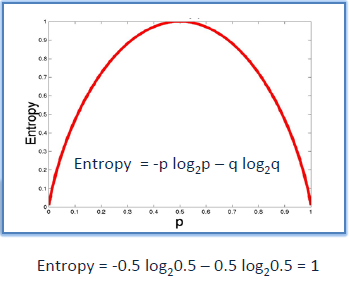
\includegraphics[width=1.00\linewidth]{images/supervised/decision_trees/entropy_1.png}
%			\caption{}
%			\label{} 
			\end{figure}
			
			
			
			\column{0.6\linewidth}
			\begin{figure}[!htbp]
				\centering
				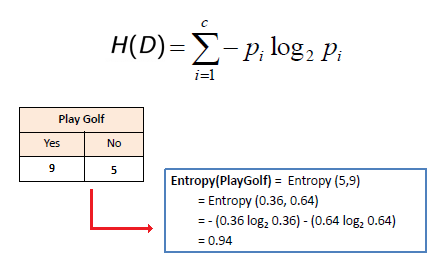
\includegraphics[width=1.0\linewidth]{images/supervised/decision_trees/entropy_2.png}
%			\caption{}
%			\label{} 
			\end{figure}
			
	\end{columns}
\end{frame}

\begin{frame}
	
	\frametitle{ID3 di \textit{Play Tennis?} 1}

	Costruiamo un albero decisionale per la tabella mostrata, usando \textbf{ID3}.\\
	L'algoritmo ID3 corrisponde all'algoritmo descritto poche slides fa, il \textbf{Build-DT}, utilizzando l'information gain per la scelta della migliore feature.
	
	\begin{figure}[!htbp]
		\centering
		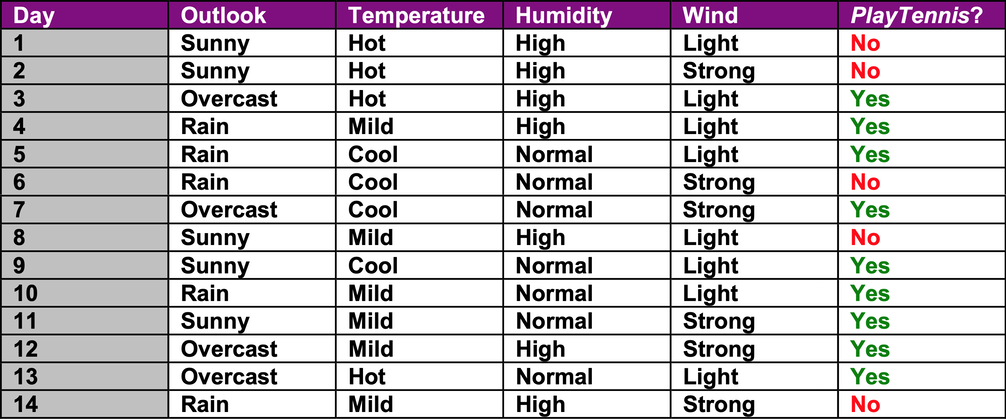
\includegraphics[width=1.00\linewidth]{images/supervised/decision_trees/example_play_tennis.png}
%		\caption{To Play or Not To Play?}
	\end{figure}
	
\end{frame}


\begin{frame}
	
	\frametitle{ID3 di \textit{Play Tennis?} 2}

	\begin{itemize}
		\item Selezioniamo l'attributo radice
		
		\begin{columns}
	
			\column{0.7\linewidth}
	%			The New York Times, July 8 1958
			\begin{figure}[!htbp]
				\centering
				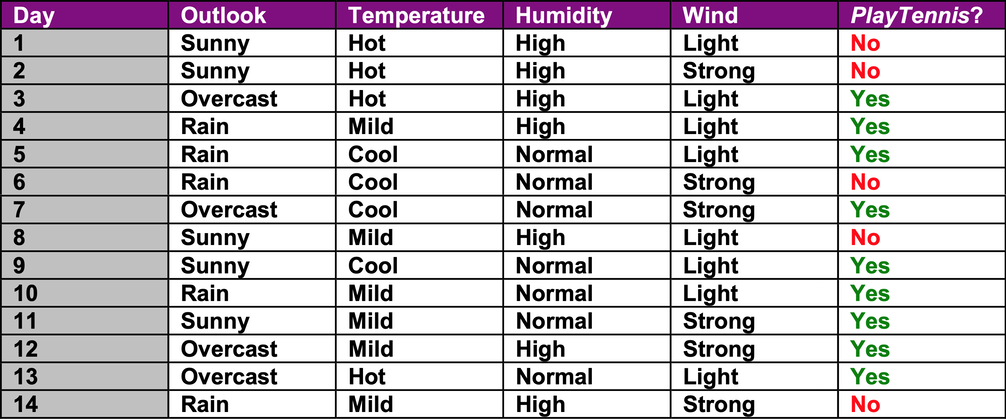
\includegraphics[width=1.00\linewidth]{images/supervised/decision_trees/example_play_tennis.png}
	%			\caption{The New York Times, July 8 1958}
				%\label{Enel_QQ_Plot_Normal} 
			\end{figure}
			
			
			
			\column{0.3\linewidth}
			\begin{figure}[!htbp]
				\centering
				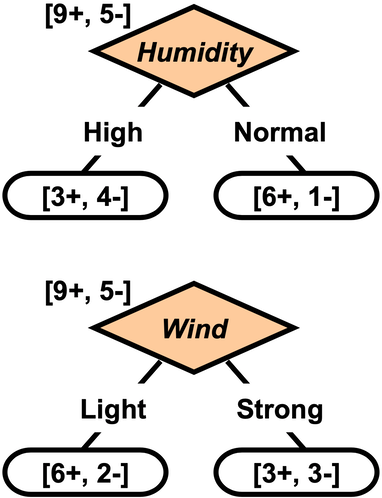
\includegraphics[width=0.75\linewidth]{images/supervised/decision_trees/example_humidity_wind.png}
	%			\caption{The New Yorker, December 6, 1958 P. 44 sopra e l'IBM 704 sotto}
				%\label{Enel_QQ_Plot_Normal} 
			\end{figure}
			
		\end{columns}
		
		
%		\item {\color{GradientDescentDiagramBlue}0.94}
%		\item {\color{GradientDescentDiagramGreen}0.985}
%		\item {\color{GradientDescentDiagramOrange}0.592}
%		\item {\color{GradientDescentDiagramRed}0.97}
		
		\item Distribuzione ``a priori'' (non condizionata): $9+$, $5-$
			\begin{itemize}
				\item[--] $\pmb{H(D)} = -\frac{9}{14} log_{2} \frac{9}{14} - \frac{5}{14} log_{2} \frac{5}{14} = \pmb{\underline{{\color{GradientDescentDiagramBlue}0.94}}}$
				\vspace{0.3em}
				\pause
				\item[--] $H(D, Humidity = High) = -\frac{3}{7} log_{2} \frac{3}{7} - \frac{4}{7} log_{2} \frac{4}{7} = {\color{GradientDescentDiagramGreen}0.985}$
				\vspace{0.3em}
				\pause
				\item[--] $H(D, Humidity = Normal) = -\frac{6}{7} log_{2} \frac{6}{7} - \frac{1}{7} log_{2} \frac{1}{7} = {\color{GradientDescentDiagramOrange}0.592}$
				\vspace{0.3em}
				\pause
				\item[--] $\pmb{\underline{Gain(D, Humidity)}} = {\color{GradientDescentDiagramBlue}0.94} + \big\{- \frac{7}{14} * {\color{GradientDescentDiagramGreen}0.985} - \frac{7}{14} * {\color{GradientDescentDiagramOrange}0.592} \big\} = \pmb{\underline{0.151}}$
				\vspace{0.3em}
				\pause
				\item[--] Analogamente,\\
					$\pmb{\underline{Gain(D, Wind)}} = {\color{GradientDescentDiagramBlue}0.94} + \big\{ -\frac{8}{14} * 0.811 - \frac{6}{14} * 1.0 \big\} = \pmb{\underline{0.048}}$
			\end{itemize}
	\end{itemize}
	
\end{frame}


\begin{frame}
	
	\frametitle{ID3 di \textit{Play Tennis?} 3}

	\begin{itemize}
		\item Selezioniamo l'attributo radice
		
		\begin{columns}
	
			\column{0.7\linewidth}
	%			The New York Times, July 8 1958
			\begin{figure}[!htbp]
				\centering
				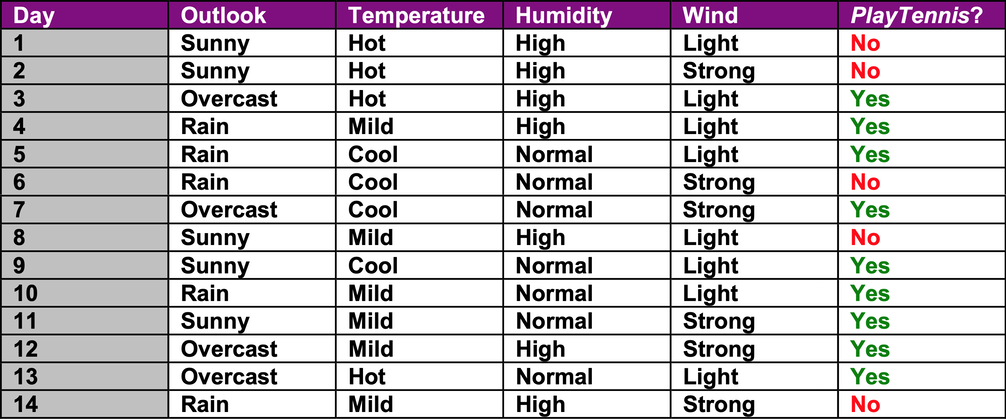
\includegraphics[width=1.00\linewidth]{images/supervised/decision_trees/example_play_tennis.png}
	%			\caption{The New York Times, July 8 1958}
				%\label{Enel_QQ_Plot_Normal} 
			\end{figure}
			
			
			
			\column{0.3\linewidth}
			\begin{figure}[!htbp]
				\centering
				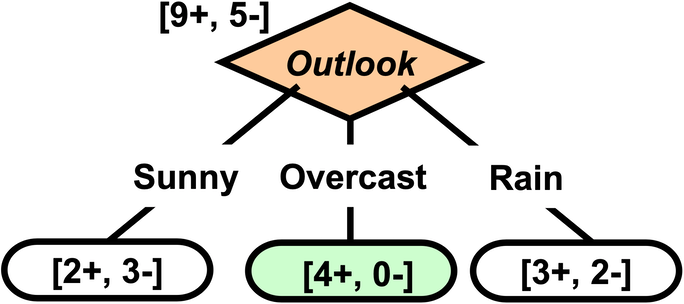
\includegraphics[width=1.1\linewidth]{images/supervised/decision_trees/example_humidity_outlook.png}
	%			\caption{The New Yorker, December 6, 1958 P. 44 sopra e l'IBM 704 sotto}
				%\label{Enel_QQ_Plot_Normal} 
			\end{figure}
			
		\end{columns}
		
		\begin{itemize}
			\item[--] $Gain(D, Humidity) = 0.151$
			\item[--] $Gain(D, Wind) = 0.048$
			\item[--] $Gain(D, Temperature) = 0.029$
			\item[--] $Gain(D, \pmb{\underline{Outlook}}) = \pmb{\underline{0.246}}$
		\end{itemize}
		
		
		\item Selezione del prossimo nodo (la radice del sottoalbero)
			\begin{itemize}
				\item[--] Continua fino a quando ogni esempio è incluso nei cammini o la purezza è del 100\%
				%\item[--] Che significa purezza = 100\%?
				%\item[--] Possiamo avere Gain(D, F) < 0?
			\end{itemize}
		
	\end{itemize}
	
\end{frame}


\begin{frame}
	
	\frametitle{ID3 di \textit{Play Tennis?} 4}

	\begin{itemize}
		\item Selezione del prossimo attributo (la radice del sottoalbero)
		
		\begin{columns}
	
			\column{0.7\linewidth}
	%			The New York Times, July 8 1958
			\begin{figure}[!htbp]
				\centering
				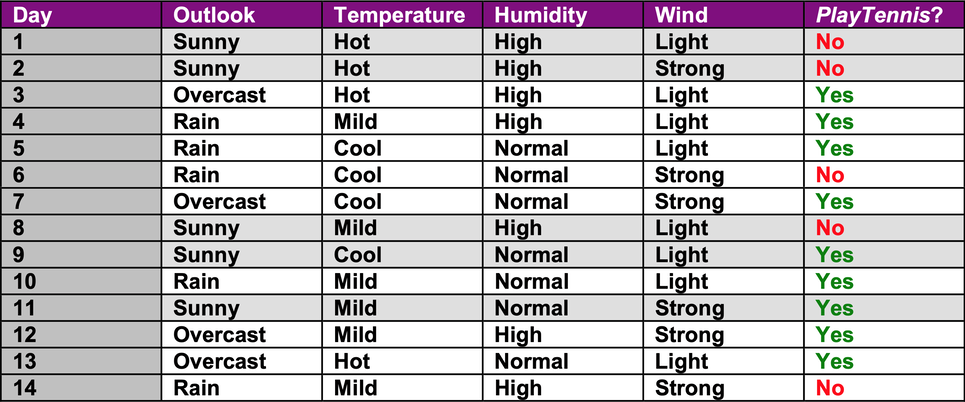
\includegraphics[width=1.00\linewidth]{images/supervised/decision_trees/example_play_tennis_sunny.png}
	%			\caption{The New York Times, July 8 1958}
				%\label{Enel_QQ_Plot_Normal} 
			\end{figure}
			
			
			
			\column{0.3\linewidth}
			\begin{figure}[!htbp]
				\centering
				%\includegraphics[width=1.1\linewidth]{images/supervised/decision_trees/example_humidity.png}
	%			\caption{The New Yorker, December 6, 1958 P. 44 sopra e l'IBM 704 sotto}
				%\label{Enel_QQ_Plot_Normal} 
			\end{figure}
			
		\end{columns}
		
		\begin{itemize} 
			\vspace{0.3em}
			\item[--] convenzione: $log_{2} (0/a) = 0$
			\vspace{0.3em}
 			\item[--] $H(D_{Sunny}) = -\frac{2}{5} log_{2} \frac{2}{5} - \frac{3}{5} log_{2} \frac{3}{5} = \pmb{\underline{{\color{GradientDescentDiagramRed}0.97}}}$
			\vspace{0.3em}
 			\item[--] $Gain(D_{Sunny}, Humidity) = {\color{GradientDescentDiagramRed}0.97} + \big\{ -\frac{3}{5} * 0 - \frac{2}{5} * 0 \big\} = \pmb{\underline{0.97}}$
 			\vspace{0.3em}
			\item[--] $Gain(D_{Sunny}, Wind) = {\color{GradientDescentDiagramRed}0.97} + \big\{ -\frac{2}{5} * 1 -\frac{3}{5} * 0.92 \big\} = 0.02$
			\vspace{0.3em}
			\item[--] $Gain(D_{Sunny}, Temperature) = 0.57$
		\end{itemize}
%		
%		
%		\item Selezione del prossimo nodo (la radice del sottoalbero)
%			\begin{itemize}
%				\item[--] Continua fino a quando ogni esempio è incluso nei cammini o la purezza è del 100\%
%				%\item[--] Che significa purezza = 100\%?
%				%\item[--] Possiamo avere Gain(D, F) < 0?
%			\end{itemize}
		
	\end{itemize}
	
\end{frame}


\begin{frame}
	
	\frametitle{ID3 di \textit{Play Tennis?} 5}
	
	\begin{figure}[!htbp]
		\centering
		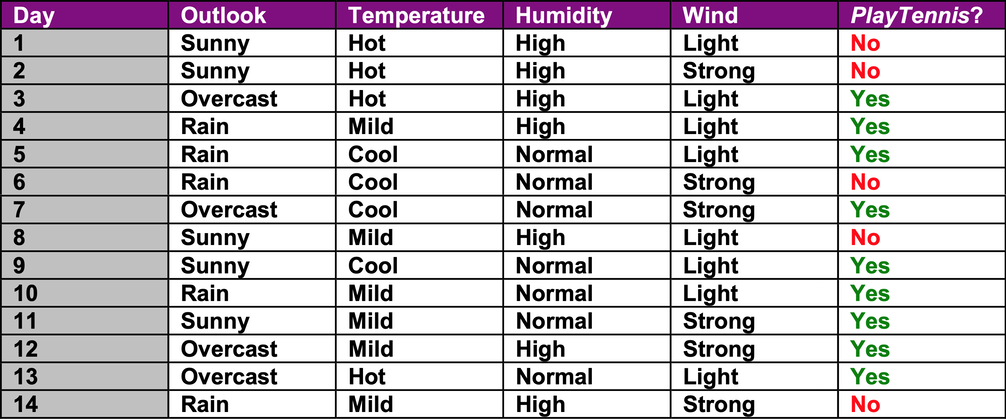
\includegraphics[width=0.65\linewidth]{images/supervised/decision_trees/example_play_tennis.png}
%		\caption{}
	\end{figure}
	
	\begin{figure}[!htbp]
		\centering
		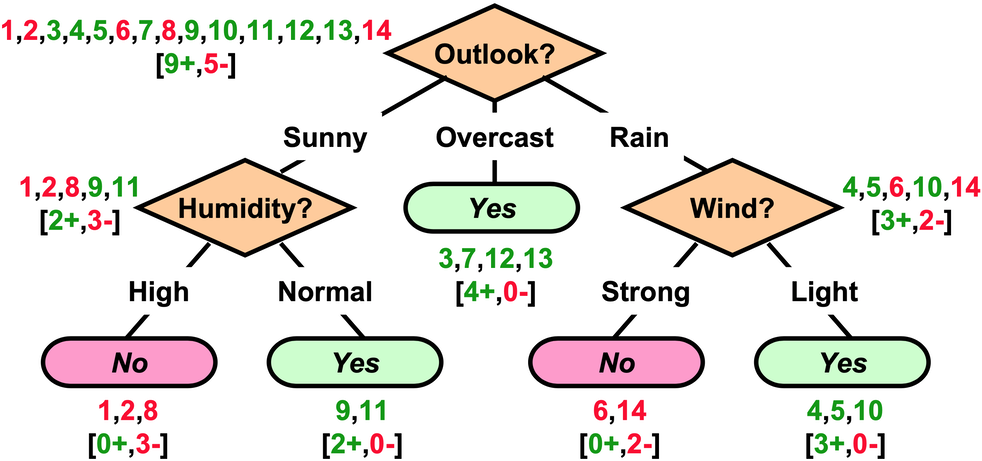
\includegraphics[width=0.65\linewidth]{images/supervised/decision_trees/example_id3_completed.png}
%		\caption{}
	\end{figure}
	
	
\end{frame}


\subsubsection[Osservazioni per la regressione]{Osservazioni per la regressione}
\begin{frame}
	
	\frametitle{Alberi decisionali per la regressione}
	
	Secondo un ragionamento simile a quanto visto per la \textbf{classificazione} è possibile costruire alberi decisionali per la \textbf{regressione}.\\
	Tuttavia saranno presenti alcune differenze significative circa i criteri con il quale selezionare la \textbf{feature ``migliore''}, circa la scelta delle \textbf{soglie di split} e circa i \textbf{criteri di arresto} da applicare durante la costruzione dell'albero.
	\newlinedouble
	
	\begin{figure}[!htbp]
		\centering
		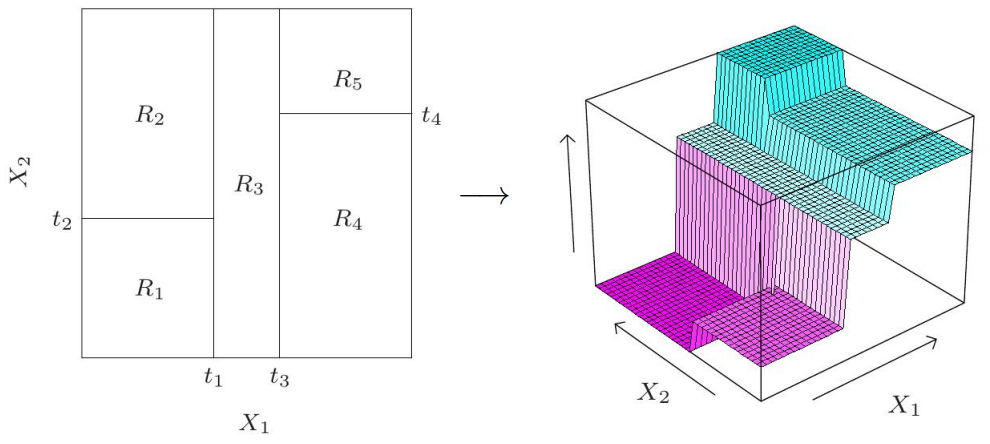
\includegraphics[width=0.7\linewidth]{images/supervised/decision_trees/regression_tree_example.png}
%		\caption{}
	\end{figure}
	
\end{frame}



\ifthenelse{\boolean{highschool}}{}{

\begin{frame}
	\frametitle{Alberi decisionali per la regressione}
	
	\begin{enumerate}
		\item Dividiamo lo spazio delle features $\mathcal{X}$ in $K$ regioni distinte e non sovrapposte $R_1,R_2,\ldots,R_K$
		\item Per ogni $x_i \in R_k$ la previsione è sempre la stessa:
			\[
				\widehat y_i = \sum_{k=1}^K \widehat y_{R_k} \mathbb{I}(x_i \in R_k) \quad \text{ dove spesso } \quad \widehat{y}_{R_k} = \frac{\sum_{i=1}^n y_i \mathbb{I}(x_i\in R_k)}{\sum_{i=1}^n \mathbb{I}(x_i\in R_k)}
			\]
	\end{enumerate}
	
	\begin{itemize}
		\item Questa scelta è analoga a quella alla base delle approssimazioni costanti a tratti o all'approccio KNN, ma la partizione di $\mathcal{X}$:
			\begin{itemize}
				\item[--] non è scelta a priori
				\item[--] non dipende dal punto in corrispondenza del quale vogliamo calcolare la previsione
				\item[--] in linea di principio, le regioni $R_k$ possono avere forma qualsiasi
			\end{itemize}
	\end{itemize}
\end{frame}


\begin{frame}
	\frametitle{Rettangoli}
	
	\begin{itemize}
		\item In assenza di vincoli, è praticamente impossibile trovare la partizione ottimale ($K$ e $R_k$, $k=1,\ldots,K$)
		\item Per semplificare il problema, assumiamo che le regioni $R_k$ siano ``iper-rettangoli''
		\item Problema: Trovare la partizione ottimale; in altre parole, quella che minimizza la SQR $\sum_{i=1}^n (y_i - \widehat y_i)^2$
		\item Anche questo problema è troppo difficile. Esistono troppe possibili partizioni in $K$ rettangoli, per ogni $K$
		\item Soluzione (simile alla \emph{forward stepwise selection}): usare un algoritmo \emph{di suddivisione ricorsivo} (\emph{Recursive Binary Splitting}, RBS)
			\begin{itemize}
				\item[--] RBS è \emph{sequenziale} -- un $X_j$ alla volta
				\item[--] Ad ogni passo viene effettuata la \emph{migliore} suddivisione sulla base dell'effetto \emph{immediato} -- un algoritmo non prospettico (in gergo, \emph{greedy} -- ingordo)
			\end{itemize}
	\end{itemize}
\end{frame}


\begin{frame}
	\frametitle{Algoritmo}
	
	\begin{enumerate}
		\item Iniziamo con la previsione $\overline y$ e SQR $\sum_{i=1}^n (y_i-\overline y)^2$
		\item Selezioniamo $X_j$ e $s$ tali che:
			\begin{itemize}
				\item Dividendo $\mathcal{X}$ in $R_{j-} = \{X|X_j < s\}$ e $R_{j+} = \{X|X_j \geq s\}$
				\item Usando $\overline y_{R_{j-}}$ e $\overline y_{R_{j+}}$ come previsioni di $Y$ su $R_{j-}$ e $R_{j+}$
			\end{itemize}
			\emph{massimizziamo la riduzione della SQR}
		\item Ripetiamo il passo 2, selezionando $X_j$, $s$  e una delle regioni identificate ai passi sucessivi
		\item Il processo continua fino a quando viene soddisfatto un criterio di arresto. Per esempio possiamo continuare fino a quando:
			\begin{itemize}
				\item[--] nessuna regione contiene più di (per esempio) cinque osservazioni
				\item[--] nessun nodo ha devianza ($=$ SQR) maggiore di una (piccola) frazione della devianza del nodo radice (di solito l'1\%)
				\item[--] il numero di suddivisioni ottimizza un criterio regolarizzzato come $\mbox{SQR}+\lambda |T|$, dove $|T|$ è il numero di ``foglie''
			\end{itemize}
	\end{enumerate}
	\begin{itemize}
		\item Il risultato finale è una funzione costante a tratti molto flessibile
		%\item Le proprietà di questo algoritmo sono essenzialmente ignote; per esempio, non sono disponibili standard error e intervalli di previsione
	\end{itemize}
\end{frame}

}

\begin{frame}
	\frametitle{Vantaggi e svantaggi}
	
	\begin{itemize}
		\item [\bb{+}] Gli alberi sono semplici
			\begin{itemize}
				\item è possibile tracciarne il grafico
				\item sono facili da interpretare
				\item sono facili da spiegare
				\item imitano il modo di ragionare delle persone
			\end{itemize}
		\item [\bb{+}] Gli alberi funzionano bene anche per $p$ elevato
		\item [\bb{+}] Gli alberi forniscono approssimazioni non parametriche flessibili
		\item [\bb{+}] Gli alberi sono facili da estendere a problemi di classificazione
	\end{itemize}
	
	\begin{itemize}
	
		\item [\bb{\mbox{$-$}}] Di solito non funzionano altrettanto bene di altri metodi avanzati
	\end{itemize}
\end{frame}


% TODO fare una sezione futura di miglioramento degli alberi, che parte con il pruning e va avanti con bagging e boosting e random forest etc...